\documentclass[fr]{../../../eplsummary}
\usepackage{../../../eplunits}
\usepackage{../../../eplmath}
\usepackage{multirow}

\newcommand\fv[1]{{\bf #1}} % free vector
\usepackage{graphicx}
\usepackage{listings}
\usepackage[autolanguage, np]{numprint}
\DeclareMathOperator{\dist}{dist}
\renewcommand{\arraystretch}{2}

\hypertitle{M\'ethodes num\'eriques}{2}{EPL}{1104}
{Beno\^it Legat\and Antoine Paris\and Gilles Peiffer}
{Vincent Legat}

\definecolor{dkgreen}{rgb}{0.25,0.7,0.35}
\definecolor{dkred}{rgb}{0.7,0,0}
\lstset{language={octave},numbers=left,numberstyle=\tiny\color{gray},
basicstyle=\rm\footnotesize,keywordstyle=\bfseries\color{dkred},frame=single,
commentstyle=\color{gray}=small, stringstyle=\color{dkgreen}}

% there ought to be a better place for this
\begin{mydef}[Grand ordre]
  On dit qu'une fonction $f(h)$ est un grand ordre de $h^n$ au voisinage
  de 0 s'il existe une constante $C$ telle que
  \[ |f(h)| \leq C |h^n| \]
  au voisinage de 0.
  On écrit alors $f(h) = \bigoh(h^n)$.
\end{mydef}

\part{Approximation numérique}
Soit une fonction $u(x)$.
Le problème d'approximation correspond à trouver une fonction
$u^h(x)$ qui approxime la fonction $u(x)$.

Cette approximation est faite à l'aide de \emph{fonctions de base} $\phi_j(x)$.
On cherche à approximer $u(x)$ avec une combinaison linéaire des $\phi_j(x)$:
\[ u(x) \approx u^h(x) = \sum_{j=1}^n a_j \phi_j(x). \]

On définit l'\emph{erreur d'approximation} $e^h(x) \eqdef u(x) - u^h(x)$.
On définit également l'\emph{ordre} d'une approximation comme étant l'ordre de
l'erreur $e^h(x)$.

\section{Interpolation}
Une interpolation est une approximation passant par certains points de $u(x)$.

Soit $(X_i, U_i)$ avec $i = 0, 1, 2, \ldots, n$ ces points. On a

\[\begin{bmatrix}
	\phi_0(X_0) & \phi_1(X_0) & \cdots & \phi_n(X_0)  \\
	\phi_0(X_1) & \phi_1(X_1)	& \cdots & \phi_n(X_1)  \\
	\vdots			& \vdots 			& 			 & \vdots \\
	\phi_0(X_n) & \phi_1(X_n)	& \cdots & \phi_n(X_n)
\end{bmatrix}
\begin{bmatrix}
	a_0 			\\
	a_1 			\\
	\vdots	\\
	a_n
\end{bmatrix}
=
\begin{bmatrix}
	U_0 			\\
	U_1 			\\
	\vdots	\\
	U_n
\end{bmatrix}.\]

En prenant $\phi_j(x) = x^j$, ça donne un système linéaire à résoudre:

\[\begin{bmatrix}
	1 			& X_0 		& \cdots & X_0^n  \\
	1 			& X_1 		& \cdots & X_1^n  \\
	\vdots	& \vdots 	& 			 & \vdots \\
	1 			& X_n 		& \cdots & X_n^n
\end{bmatrix}
\begin{bmatrix}
	a_0 			\\
	a_1 			\\
	\vdots	\\
	a_n
\end{bmatrix}
=
\begin{bmatrix}
	U_0 			\\
	U_1 			\\
	\vdots	\\
	U_n
\end{bmatrix}.\]

On voit que la matrice des coefficients du système (appelée la \textit{matrice
de Vandermonde}) est régulière.

Ce qui nous donne le théorème suivant.
\begin{mytheo}
  Il existe un et un seul polynôme d'interpolation de degré $n$ passant
  par $n+1$ points d'abscisses distinctes.
\end{mytheo}

\subsection{Formule d'interpolation de Lagrange}
Au lieu de résoudre le système précédent, la formule d'interpolation
de Lagrange nous permet d'obtenir directement cet unique polynôme
d'interpolation.

Il suffit de prendre
\[
  \phi_j(x) = \frac{\prod_{i \neq j} (x - X_i)}
  {\prod_{i \neq j} (X_j - X_i)}.
\]

\begin{figure}[ht]
	\centering
	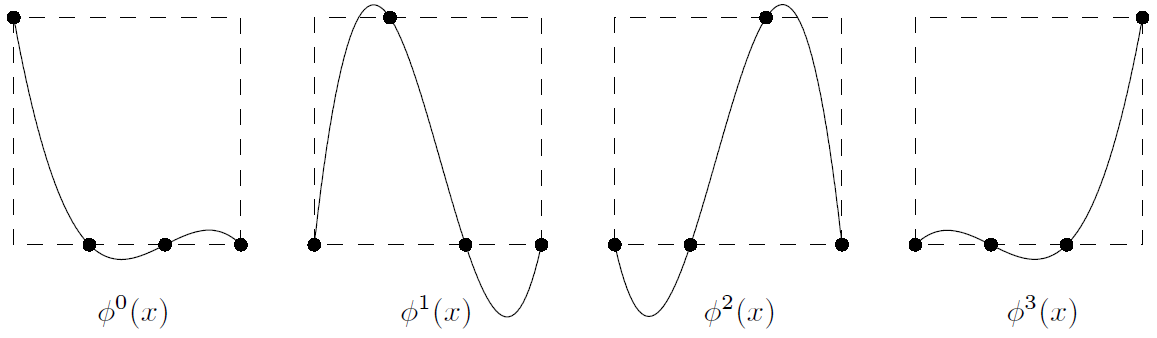
\includegraphics[scale=0.6]{img/fonctions_lagrange.png}
	\caption{Les fonctions de base de Lagrange pour les abscisses $X_0 = 0$,
	$X_1 = \frac{1}{3}$, $x_2 = \frac{2}{3}$ et $X_3 = 1$ sur l'intervalle
	$[0,1]$. (Tiré du syllabus.)}
	\label{fig:lagrange}
\end{figure}

On remarque alors que la matrice de Vandermonde devient la matrice
identité et que $a_j = U_j$. En effet, $\phi_i(X_j) = 0$ $\forall i \neq j$
et $\phi_i(X_i) = 1$ (voir \figuref{lagrange}).

\subsection{Interpolation en 2D}
(Voir APE1, exercice 12.) On peut étendre la notion d'interpolation à des fonctions à deux variables. Imaginons
par exemple que l'on veuille interpoler une fonction $u(x, y)$ par une fonction $u^h(x, y)$
sur un domaine carré sur lequel on connait la valeur de $u$ aux quatres sommets : $u(X_i, Y_i) = U_i$,
$i = 0, 1, 2, 3.$ On pourrait prendre comme fonctions de bases les monômes $1$, $x$, $y$ et $xy$
de sorte que $u^h(x, y) = a_0 + a_1x + a_2y + a_3xy$ et résoudre le système linéaire qui en découle.
Mais on peut faire mieux. Pour ce faire, on généralise la notion de fonction de base de Lagrange au
cas à deux dimensions.

\[ u(x, y) \approx u^h(x, y) = \sum U_i \phi_i(x, y) \]

où

\[ \phi_j(x) = \frac{\prod_{i \neq j} (x - X_i)(y - Y_i)}
  {\prod_{i \neq j} (X_j - X_i)(Y_j - Y_i)}. \]

On a donc bien $\phi_i(X_i, Y_i) = 1$ et $\phi_i(X_j, Y_j) = 0 \forall j\neq i$.

\subsection{Erreur d'interpolation}
L'erreur d'interpolation du polynôme de Lagrange peut être calculée
par le Théorème~\ref{thm:error}.
\begin{mytheo}
  \label{thm:error}
  Soit $X_0 < X_1 < \ldots < X_n$ les abscisses des points d'interpolation.
  Si la fonction $u(x)$ est définie sur l'intervalle $\intervalcc{X_0}{X_n}$ et qu'elle
  est $(n+1)$ fois dérivable sur $\intervaloo{X_0}{X_n}$, alors pour tout
  $x \in \intervaloo{X_0}{X_n}$, il existe $\xi(x) \in \intervaloo{X_0}{X_n}$ tel que
  \[ e^h(x) = \frac{u^{(n+1)}(\xi(x))}{(n+1)!}
  \prod_{i=0}^n (x - X_i). \]
\end{mytheo}

\begin{myrem}\label{rem:borne}
	En pratique on ne dispose pas de $u(x)$ et de $\xi(x)$, on ne dispose donc
	pas non plus de $u^{(n+1)}(\xi(x)$). On va donc introduire une constante
	$C$ qui borne toutes les dérivées de $u(x)$ (dans certains cas c'est très simple, comme
	pour $\sin(x)$ ou $\cos(x)$ dont la dérivée d'ordre $n+1$ sera comprise
	entre $-1$ et 1). Il est également possible de démontrer que $\prod_{i=0}^n (x - X_i)
	< n! \frac{h^{n+1}}{4}$ où $h$ est le pas entre les abscisses $X_i$ (voir APE1, question 5).
	On peut donc finalement écrire

	\[ \abs{e^h(x)} \leq \frac{C}{(n+1)!} \cdot n! \frac{h^{n+1}}{4} = \frac{C}{4(n+1)}h^{n+1}. \]

  $e^h(x)$ est donc d'ordre $n+1$, $e^h(x) = \bigoh(h^{n+1})$.
\end{myrem}

\subsection{Convergence de l'interpolation polynomiale}
\begin{mydef}[Convergence d'une interpolation]
	Une interpolation est dite convergente si l'erreur d'interpolation tend vers
	zéro lorsque le nombre de degrés de liberté, c'est à dire $n$ tend vers l'infini :

	\[ \lim_{n \to \infty} e^h(x) = 0 \]

	pour $x \in \intervalcc{X_0}{X_n}$.
\end{mydef}

Comme on peut le voir au travers de la remarque \ref{rem:borne}, on peut prouver
ce résultat de convergence pour des fonctions $u(x)$ dont les dérivées sont
bornées sur le domaine d'interpolation par une constante $C$ (e.g $\sin(x)$, $\cos(x)$, $\e^x$).
En effet, en se rappelant que $h = \frac{b-a}{n}$, on a bien

\[ \lim_{n \to \infty} e^h(x) = C \lim_{n \to \infty} \frac{1}{4(n+1)}\left(\frac{b-a}{n}\right)^{n+1} = 0. \]

\subsection{Les abscisses de Tchebychev}
Pour certaines fonctions $u(x)$ plus ou moins irrégulières (e.g fonctions de Runge),
l'interpolation ne converge pas lorsque le nombre de points d'interpolation
augmente : il y a présence de fortes oscillations de l'interpolant près des
bords de l'intervalle d'interpolation lorsque le degré $n$ augmente (à cause de
la dérivée d'ordre élevé dans la borne de l'erreur).
On peut réduire l'erreur maximale en essayant de la répartir le plus possible.
Comme c'est au bord qu'il y a le plus d'erreur, l'idée serait de mettre
plus de points au bord.
Pour cela, il suffit d'utiliser les abscisses de Tchebychev:
\[ X_i = \cos\left(\frac{(2i+1)\pi}{2(n+1)}\right). \]

\subsection{Les splines cubiques}
L'utilisation des abscisses de Tchebychev ne suffit parfois pas à faire converger
l'interpolation polynomiale (c'est le cas pour des fonctions pas du tout régulières),
il faut alors utiliser une autre méthode : l'interpolation polynomiale par morceaux.
Au lieu de chercher un polynôme passant par tous les points, l'idée des
splines cubiques est de prendre un polynôme différent entre chaque paire
de points adjacents.

On définit donc $n$ polynômes cubiques $u^{h_i}$, chacun dans son
intervalle $\intervalcc{X_{i-1}}{X_i}$.
On peut déterminer $4n-2$ coefficients grâce à $4n-2$ équations.
\begin{itemize}
  \item Passer par tous les points: $2n$ équations;
  \item Dérivées premières et secondes égales aux points $X_i$
    pour deux polynômes $u^{h_i}$ adjacents: $2n-2$ équations.
\end{itemize}

Comme on a $4n$ coefficients à déterminer, on peut rajouter deux contraintes.
On les rajoute souvent sur $u^{h_1}(x)$ en $X_0$ et sur $u^{h_n}(x)$ en $X_n$
ou sur leurs dérivées en ces points.

\section{Approximation}
Il est parfois préférable de ne pas imposer que la fonction passe par tous les
points car dans ce cas, on n'a plus une interpolation.

\subsection{Approximation au sens des moindres carrés}
Il y a 2 cas, soit on connait $n+1$ points de $u(x)$, soit on
connait carrément $u(x)$ entre $a$ et $b$.
L'analyse de ces cas est assez semblable, pour passer du second au premier,
il suffit de discrétiser les intégrales en somme sur les points qu'on connait.
Faisons donc uniquement l'analyse dans le deuxième cas.

On cherche donc à minimiser
\[ \int_a^b \left(e^h(x)\right)^2 \dif x =
\int_a^b \left(u(x) - u^h(x)\right)^2 \dif x. \]

Seulement, on remarque qu'en définissant le produit scalaire
$\langle f, g \rangle = \int_a^b fg \dif x$, ce qu'on doit minimiser devient
\[ \norm{e^h(x)} = \norm{u(x) - u^h(x)}. \]

C'est à dire qu'on cherche une fonction $u^h(x)$ dans l'espace euclidien
formé par les combinaisons linéaires des fonctions $\phi_j(x)$ qui soit
à une distance minimale de $u(x)$ selon le produit scalaire défini pour
cet espace.

$u^h(x)$ est donc la projection orthogonale de $u(x)$ dans cet espace.
$e^h(x)$ est donc orthogonal à cet espace.
D'où $\langle \phi_k, e^h \rangle = 0$ pour $k = 0, 1, \ldots, n$.
Ce qui nous permet de trouver que
\[ \sum_{j=0}^n \left(a_j \int_a^b \phi_k(x) \phi_j(x) \dif x\right)
= \int_a^b \phi_k(x) u(x) \dif x, \]

en prenant des $\phi_j$ orthogonaux, comme $\phi_j(x) = \cos\left((j+1)x\right)$.
On peut calculer $a_j$ plus facilement en projettant $u$ sur $\phi_j$.
Attention néanmoins car si les $\phi_j$ sont orthogonaux,
ils ne sont pas nécessairement orthonormés !
On a donc
\[ a_j = \frac{1}{\pi} \langle u, \phi_j \rangle =
\frac{1}{\pi} \int_{-\pi}^{\pi} u(x) \cos((j+1)x) \dif x. \]

\subsection{Les B-splines et les NURBS}
Les B-splines et les NURBS servent à faire une approximation
de $n+1$ points $(X_i, Y_i)$.
Cette approximation est paramétrée en fonction de $t$.
On donne alors $n+1$ noeuds
\[ T_0 \leq T_1 \leq \ldots T_n. \]
On voit ici qu'on se permet de mettre plusieurs noeuds au même $t$.

\section{Les fonctions B-splines}
Une fonction B-spline est définie comme suit
\[ B_i^p(t) = \frac{t-T_i}{T_{i+p}-T_i} B_i^{p-1}(t)
+ \frac{T_{i+1+p} - t}{T_{i+1+p} - T_{i+1}}B_{i+1}^{p-1}(t) \]
où, si un dénominateur s'annule, on met le terme à 0.

L'initialisation est la suivante
\[ B_i^0(t) = \left\{\begin{array}{ll}
1 & \text{si }t \in [T_i, T_{i+1}[\\
0 & \text{sinon.}\end{array}\right.. \]

On peut déduire de cette définition le théorème suivant
\begin{mytheo}
  \label{thm:sumbspline1}
  À l'exclusion des $p$ premiers et $p$ derniers intervalles,
  la somme des B-splines vaut l'unité.
  \[ \sum_{i=0}^{n-p-1} B_i^p(t) = 1 \]
  où $T_p \leq t < T_{n-p}$.
\end{mytheo}

On peut ensuite calculer l'approximation avec la formule suivante
\[ (x^h(t), y^h(t)) = \sum_{i=0}^{n-p-1} B_i^p(t) (X_i, Y_i) \]

\section{Les NURBS (Non-Uniform Rational B-splines)}
Pour être capable de représenter exactement certaines formes telles
que les coniques, on a rajouté la possibilité de rajouter des poids $W_i$.
La formule de l'approximation devient alors
\[ (x^h(t), y^h(t)) =
\frac{\sum_{i=0}^{n-p-1}W_iB_i^p(t)(X_i, Y_i)}
{\sum_{i=0}^{n-p-1}W_iB_i^p(t)}. \]

En se rappelant du Théorème~\ref{thm:sumbspline1}, on voit
qu'une B-spline est le cas particulier des NURBS où tous les $W_i$ valent 1.

\part{Intégration numérique}
Soit une fonction $u(x)$.
Une intégrale classique requiert la primitive de $u(x)$.
Seulement, cette méthode est souvent assez fastidieuse à effectuer
numériquement.

L'intégration numérique se fait à partir de différents points $X_i$ auquels
on donne un poids $w_i$. On utilise ensuite la formule suivante
\[ \int_a^b u(x) \dif x = I \approx I^h = \sum_{i=0}^m w_i u(X_i). \]

qu'on appelle règle d'intégration ou \emph{quadrature}.
Si $X_0 = a$ et $X_m = b$, on dit que la méthode est \emph{fermée},
sinon, on dit qu'elle est \emph{ouverte}.

On définit l'\emph{erreur d'intégration} $E^h \eqdef I - I^h$.
On définit également le \emph{degré de précision} d'une méthode d'intégration
numérique comme le plus grand entier $d$ tel que pour tout polynôme de degré
inférieur où égal à $d$, $E^h = 0$.

Sans perte de généralité, on peut toujours se ramener à une intégrale
sur l'intervalle $\intervalcc{-1}{1}$. Il suffit pour cela d'utiliser un changement
de variable
\[ I = \int_a^b u(x) \dif x =
\frac{b-a}{2} \int_{-1}^1 u(x(\xi)) \dif \xi, \]

où $x(\xi) = \frac{b-a}{2}\xi + \frac{b+a}{2}$.
Par exemple, si $u(x) = x^2$, $a = 0$ et $b = 1$,
on a $x(\xi) = \frac{\xi+1}{2}$ et donc $\dif x = \frac{1}{2}\dif \xi$ d'où
\[ \int_0^1 x^2 \dif x =
\frac{1}{2}\int_{-1}^1 \left(\frac{\xi+1}{2}\right)^2 \dif \xi. \]

On va donc se limiter par la suite à l'intégration de fonction entre $-1$ et 1.

\section{Newton-Cotes: Méthodes à pas égaux}
La méthode de Newton-Cotes revient à calculer l'intégrale de $u^h$ au lieu
de $u$ qui est son interpolation par des points équidistants.
\[ I^h = \int_{-1}^1 u^h(x) \dif x =
\sum_{i=0}^m u(X_i) \int_{-1}^1 \phi_i(x) \dif x.\]
On a donc $w_i = \int_{-1}^1 \phi_i(x) \dif x$.
Comme ils ne dépendent pas de $u$, on peut les calculer à priori.

On remarque que si $u$ est un polynôme de degré $m$, $E^h = 0$.
Mais comme $\int_{-1}^1 x^{2n+1} \dif x = 0$ $\forall n \in \mathbb{N}$,
si $m$ est pair et que $u$ est un polynôme de degré $m+1$,
on a aussi $E^h = 0$. Ceci permet d'expliquer pourquoi le degré
de précision de la méthode de Simpson est 3, alors qu'on utilise
un polynôme de degré 2 comme interpolation de $u$.

On a donc le tableau suivant où $d$ est le degré de précision de la méthode.
\begin{center}
  \begin{tabular}{c|c|c}
    $m$ & Nom de la méthode & $d$\\
    \hline
    1 & Trapèzes & 1\\
    2 & Simpson & 3\\
    3 & Simpson $\frac{3}{8}$ & 3\\
    4 & Boole & 5\\
  \end{tabular}
\end{center}

\begin{figure}[ht]
	\centering
	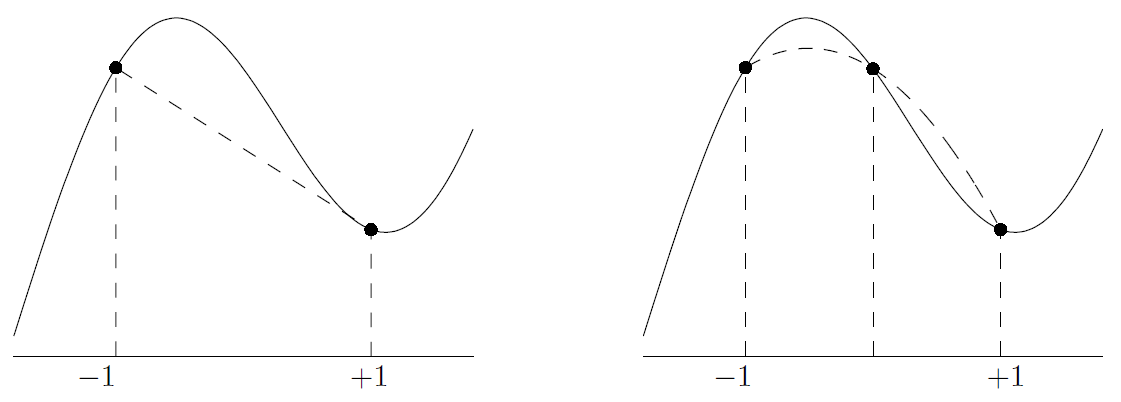
\includegraphics[scale=0.6]{img/trapezes_simpson.png}
	\caption{Interprétation géométrique de la méthode des trapèzes et de
	la méthode de Simpson. (Tiré du syllabus.)}
	\label{fig:trapeze-simpson}
\end{figure}

\subsection{Méthodes composites}
On a des méthodes efficaces pour calculer l'intégrale sur plusieurs
intervalles juxtaposés mais si on augmente trop $m$, on aura le même problème
que pour l'interpolation, l'erreur deviendra très importante pour un bon
nombre de $u$.

L'idée est donc de séparer l'intervalle à intégrer en un certain nombre
de fois $m$ intervalles qu'on intégrera séparément.

Pour cela, il est intéressant de calculer l'expression des $w_i$
en fonction de $h$, l'écart entre deux abscisses consécutives.
On a pour les méthodes avec $m = 1, 2, 4$, respectivement,
\begin{align*}
  \int_{-h/2}^{h/2}u(x)\dif x & =
  \frac{h}{2} \left(U_{-h/2} + U_{h/2}\right)
  -\frac{h^3}{12}u^{(2)}(\xi)\\
  \int_{-h}^{h}u(x)\dif x & =
  \frac{h}{3} \left(U_{-h} + 4 U_0 + U_{h}\right)
  -\frac{h^5}{90}u^{(4)}(\xi)\\
  \int_{-2h}^{2h}u(x)\dif x & =
  \frac{2h}{45}
  \left(7U_{-2h} + 32U_{-h} +12U_0 + 32U_{h} + 7U_{2h}\right)
  -\frac{8h^7}{945}u^{(6)}(\xi).
\end{align*}
Les termes en $h^3$, $h^5$ et $h^7$ sont les erreurs \emph{locales}
sur un sous-intervalle.

\paragraph{Attention}
Dans les équations précédentes, $h = (b-a), \frac{b-a}{2}, \frac{b-a}{4}$
respectivement où $b-a$ est la longueur de l'intervalle.

\begin{figure}[ht]
	\centering
	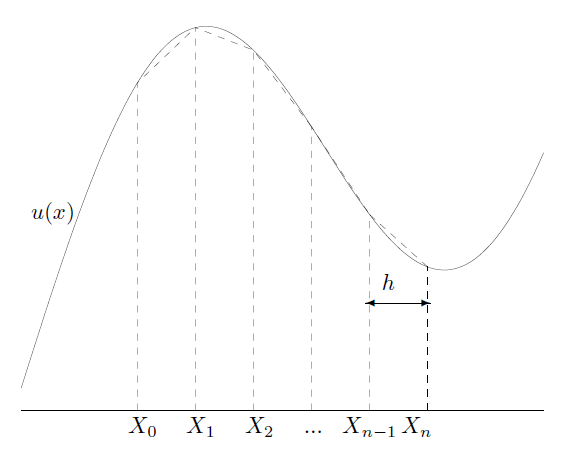
\includegraphics[scale=0.7]{img/trapezes_composites.png}
	\caption{Méthode composite des trapèzes - intervalles juxtaposés.
	(Tiré du syllabus.)}
	\label{fig:trapeze-composite}
\end{figure}

\subsection{Erreur d'interpolation}
On peut calculer l'erreur d'interpolation et obtenir les relations suivantes
pour, respectivement, $m = 1, 2, 4$.
\begin{align*}
  \abs{E^h} & \leq \frac{C_2(b-a)}{12}h^2\\
  \abs{E^h} & \leq \frac{C_4(b-a)}{180}h^4\\
  \abs{E^h} & \leq \frac{2C_6(b-a)}{945}h^6
\end{align*}
où $C_i$ est une borne de $\abs{u^{(i)}(x)}$. On remarque qu'on perd un ordre
par rapport aux erreurs locales. Prenons par exemple l'erreur locale pour
la méthode de Simpson : $E^h_\textnormal{locale} = -\frac{h^5}{90}u^{(4)}(\xi)
= \frac{h^5}{90}C_4$. L'erreur totale est obtenue en sommant les erreurs locales
des $n$ sous-intervalles :

\[ E^h = \sum_{i=0}^n E^h_{\textnormal{locale}, i}. \]

On a donc que

\[ \abs{E^h} \leq n\frac{h^5}{90}C_4. \]

Or, pour la méthode composite de Simpson, $2nh = b-a$. On a donc finalement

\[ \abs{E^h} \leq \frac{C_4(b-a)}{180}h^4 \]

où a donc bien perdu un ordre par rapport aux erreurs locales.

\section{Gauss-Legendre: Méthodes à pas inégaux}
Avec la méthode de Newton-Cotes, on sait, avec $n+1$ points, avoir
un degré de précision $d = n$ ou même $d = n+1$ si $n$ est pair.

Seulement, en se laissant $n+1$ degrés de liberté supplémentaires
qui sont les choix des abscisses, on peut atteindre
un degré de précision $d = 2n+1$.

C'est d'ailleurs la méthode utilisée pour calculer ces points.
On les prend de telle sorte que tout polynôme de degré $\leq 2n+1$ soit
intégré parfaitement.

Ça nous donne le système de $2n+2$ équations suivant à résoudre
pour trouver les $X_i$ et les $w_i$.
\begin{equation*}
  \left\{
  \begin{array}{lclc}
  \sum_{i=0}^n w_i X_i^{2j} & = & \frac{2}{2j+1} \multirow{2}{*}{\qquad pour $j = 0,\dots,n$.}\\
  \sum_{i=0}^n w_i X_i^{2j+1} & = & 0
  \end{array}
  \right.
\end{equation*}

Ce qui donne
\[
  \begin{array}{|c|c|c|}
    \hline
    n+1 & X_0, \dots, X_n & w_0, \dots, w_n\\
    \hline
    1 & 0 & 2\\
    2 & -\num{0.58}, \num{0.58} & 1, 1\\
    3 & -\num{0.77}, 0, \num{0.77} & \num{0.56}, \num{0.89}, \num{0.56}\\
    \hline
  \end{array}
\]

\section{Méthodes récursives}
\subsection{Extrapolation de Richardson}
Supposons que l'on connaisse $f(x)$ pour un certain nombre d'abscisses en
suite géométrique. On supposera ici que la raison vaut $\frac{1}{2}$.
On sait extrapoler la valeur de $f(0)$.

Supposons donc qu'on connaisse
$f(h), f\!\left(\frac{h}{2}\right), \dots, f\!\left(\frac{h}{2^n}\right)$.
Posons
$F_{i, j}$ tels que $F_{i, 0} = f\!\left(\frac{h}{2^i}\right)$ et
\[ F_{i, j} = \frac{2^j F_{i, j-1} - F_{i-1, j-1}}{2^j - 1}. \]

$F_{n, n}$ est une extrapolation d'ordre
$\bigoh\left(h^{n+1}\right)$ de $f(0)$.

Le schéma d'une extrapolation de Richardson est disponible à la
\figuref{richardson}.

\begin{figure}[!ht]
	\centering
	\begin{tikzpicture}
		\draw (0,0) node[]{$\cfrac{h}{2^0}$};
		\foreach \r in {1,2,...,5} \draw (0,-\r)node[]{$\cfrac{h}{2^{\r}}$};

		\foreach \s in {0,...,5}
		\foreach \r in {\s,...,5} {
			\draw (0.75 + 2*\s,-\r)node[]{$F_{\r,\s}$};
		}

		\foreach \r in {1,2,...,6} \draw (-1.25+\r*2,-6)node[]{$\bigoh\left(h^{\r}\right)$};

		\foreach \s in {1,...,5}
		\foreach \r in {\s,...,5} {
			\draw [->,thick] (2*\s-0.75,1-\r) -- (2*\s +0.25,-\r+0.25);
		}
		\foreach \s in {1,...,5}
		\foreach \r in {\s,...,5} {
			\draw [->,thick] (2*\s-0.75,-\r) -- (2*\s +0.25,-\r);
		}


	\end{tikzpicture}
	\caption{Extrapolation de Richardson.}
     \label{fig:richardson}
\end{figure}

% TODO : ajouter l'interprétation graphique de l'extrapolation de Richardson

\subsection{Méthode de Romberg}
Soit $f(h) = I^h$, l'intégrale exacte est $f(0)$.
On peut donc utiliser Richardson en calculant
$I^h$ avec la méthode des trapèzes.
C'est ce qu'on appelle la méthode de Romberg.

Cependant, $E^h$ n'a pas de terme d'ordre impair, on peut donc passer
une étape sur deux dans Richardson.
On utilise donc la méthode adaptée suivante pour la récurrence:
\[ I_{i, j} = \frac{2^{2j} I_{i, j-1} - I_{i-1, j-1}}{2^{2j} - 1} \]
$I - I_{n, n}$ est alors de grand ordre $\bigoh\left(h^{2(n+1)}\right)$.

\part{Dérivation numérique}
Taylor nous permet, avec un peu d'astuce, d'obtenir des
expressions pour les dérivées de $u$.
Sans perte de généralité, on va les calculer autour de 0.

\section{Différences}

\subsection{Différences centrées}
\label{sec:diffcent}
Les différences centrées sont des différences faisant
intervenir $U_{-h}$ à chaque fois qu'elles font intervenir $U_{h}$.
L'avantages c'est que, dans Taylor, tous les termes d'ordre impair
se suppriment et on peut obtenir un degré plus élevé
\begin{align*}
  u'(0) & \approx \frac{U_h - U_{-h}}{2h} & \bigoh(h^2)\\
  & \approx \frac{-U_{2h} + 8U_h - 8U_{-h} + U_{-2h}}{12h} & \bigoh(h^4).
\end{align*}

\subsection{Différences unilatérales}
Les différences unilatérales sont moins efficaces que les différences
centrées et sont utilisées quand on ne sait calculer des valeurs qu'avant
ou après 0.

\subsection{Différences amont}
\begin{align*}
  u'(0) & \approx \frac{3U_0 - 4U_{-h} + U_{-2h}}{2h} & \bigoh(h^2).
\end{align*}

\subsection{Différences aval}
\begin{align*}
  u'(0) & \approx \frac{-3U_0 + 4U_{h} - U_{2h}}{2h} & \bigoh(h^2).
\end{align*}

\paragraph{Attention}
Ces méthodes souffrent cruellement des erreurs d'arrondi
car au plus $h$ est petit, au plus $U_h - U_{-h} \ll U_h$.

\subsection{Extrapolation de Richardson}
On peut appliquer Richardson pour continuer à gagner en précision
en évitant de prendre des $h$ trop petits et d'avoir des erreurs d'arrondi.

\subsubsection{Différences centrées}
Pour les différences centrées, on sait que l'erreur ne comporte
pas de termes avec des puissances impaires de $h$.

Dès lors, il faut utiliser l'adaptation de Romberg.
\[ D_{i, j} = \frac{2^{2j}D_{i,j-1} - D_{i-1,j-1}}{2^{2j}-1}. \]
$D_{n, n}$ sera alors de grand ordre $\bigoh(h^{2(n+1)})$.

\part{Résolution numérique du problème de Cauchy}
\begin{myprob}[Problème de Cauchy]
Soit le problème de Cauchy suivant

Trouver $u(x)$ tel que
\[ \left\{ \begin{array}{rclr}
    u'(x) & = & f(x,u(x)), & x \in \intervalcc{a}{b}\\
    u(a) & = & \bar{u}.
\end{array} \right. \]
\end{myprob}
On utilise aussi souvent $\hat{f}(x) \eqdef f(x, u(x))$.

Définissons aussi la jacobienne de l'équation linéaire comme suit
\[ J(x, u(x)) \eqdef \left.\fpart{f}{u}\right|_{(x,u(x))}. \]

% TODO : arithmétique en virgule flottante

\section{Stabilité d'une équation différentielle}
Avant de regarder comment résoudre cela numériquement,
analysons comment se propage une erreur de mesure $\epsilon$.

On cherche $u_\epsilon(x)$ avec une condition initiale modifiée suivante
\[ u_\epsilon(a) = \bar{u} + \epsilon. \]
Définissons
\[ e_\epsilon(x) = u_\epsilon(x) - u(x) \]

On peut montrer que
\[ e'_\epsilon(x) \approx J(x, u(x))\cdot e_\epsilon(x). \]
C'est donc la solution du problème de Cauchy
\[ \left\{ \begin{array}{rclr}
    e'_\epsilon(x) & \approx & J(x, u(x)) \cdot e_\epsilon(x), & x \in \intervalcc{a}{b}\\
    e_\epsilon(a) & = & \epsilon.
\end{array} \right. \]

On peut donc dire que l'équation différentielle est stable lorsque
$J(x, u(x)) < 0$ et instable lorsque $J(x, u(x)) > 0$
même si ça reste une approximation.

Lorsque l'équation différentielle est instable, ça ne sert à rien
que la méthode numérique qu'on utilise pour la résoudre soit stable.

\section{Méthodes de résolution numériques}
On peut résoudre numériquement un problème de Cauchy en divisant
$\intervalcc{a}{b}$ en $m$ sous-intervalles de taille uniforme $h$.
Soit $a = X_0, X_1, \dots, b = X_m$ ces abscisses discretisées et
$\bar{u} = U_0, U_1, \dots, U_m$ les images approchées $u^h(X_i) = U_i$.

\begin{mydef}[Méthode explicite et implicite]
Une méthode est dite implicite si elle requiert le calcul de
$f(X_{i+1},U_{i+1})$ pour approximer $U_{i+1}$.
Sinon, c'est une méthode explicite.
\end{mydef}

\begin{mydef}[Ordre d'une méthode à pas séparés]
Si une méthode a une erreur locale de discrétisation d'ordre
$\bigoh(h^{n+1})$, son erreur globale sera $\bigoh(h^n)$.
\end{mydef}

\begin{mydef}[Méthode à pas liés et séparés]
Une méthode à pas liés est une méthode qui fait intervenir
plus de $U_j$ qu'uniquement $U_i$ dans le calcul de $U_{i+1}$.
Par exemple, si elle fait intervenir $U_i$ et $U_{i-1}$, elle
est à pas lié.
Sinon, elle est à pas séparés.
\end{mydef}

\begin{mydef}[Problème raide]
Un problème est raide lorsque $J(x, u(x)) \ll 0$.
Pour les problèmes raides, les méthodes implicites sont meilleures que les
méthodes explicites.
\end{mydef}

\subsection{Analyse de la stabilité}
Pour analyser la stabilité d'une méthode d'intégration numérique d'un
problème de Cauchy
\[ u' = f(x, u), \]
on analyse l'évolution de l'erreur avec la même méthode
numérique mais avec
\[ e' = \lambda e \]
et donc $f_e(x, e) = \lambda e$.
On arrive alors à une équation de récurrence homogène sur $E_i$.
On impose alors que $\lim_{n \to \infty} E_i = 0$, c'est à dire que
que toutes les $s$ racines $r_i$ du polynôme caractéristique doivent être de module plus petit que 1
car la solution de l'équation de récurrence est
\[ E_i = \sum_{i = 1}^s P_i(n)r_i^n \]
avec $P_i$ un polynôme tel que
$\deg(P_i) \leq m_i$ pour $i = 1, \dots, s$.

On fait donc un \emph{plot} du maximum des modules des racines en fonction de $h\lambda$ qui peut
être complexe car $h \in \Rplus$ et $\lambda \in \C$.

Pour qu'une méthode soit stable en $(x, u)$,
il faut alors que $\max_i \abs{r_i} < 1$ pour
$\lambda$ valant chacune des valeurs
propres de $\left.\fpart{f}{u}\right|_{(x,u)}$.

\begin{myexem}
  Par exemple, pour Crank-Nicolson, on a
  \begin{align*}
    E_{i+1} & = E_i + \frac{h}{2} (f_e(X_i, E_i) + f_e(X_{i+1}, E_{i+1}))\\
            & = E_i + \frac{h\lambda}{2} (E_i + E_{i+1})\\
            & = E_i \frac{2 + h\lambda}{2 - h\lambda}
  \end{align*}
  d'où le polynôme caractéristique
  \[ r - \frac{2 + h\lambda}{2 - h\lambda} = 0. \]
  On impose donc
  \[ \abs{\frac{2 + h\lambda}{2 - h\lambda}} \leq 1 \]
  ce qui s'interprête géométriquement comme
  $\dist(h\lambda, -2) \leq \dist(h\lambda, 2)$, d'où
  \[ \Re(h\lambda) \leq 0. \]
\end{myexem}

\subsection{Méthode de Taylor}
On remarque que, lorsqu'on connait $U_i$, on sait calculer les dérivées
successives de $u^h(X_i)$ par l'opérateur
\[ \left.\fdif{}{x}\right|_{u'=f} = \left(\fpart{}{x} + f\fpart{}{u}\right). \]

La méthode de Taylor consiste à appliquer Taylor d'un certain degré.
Par exemple, pour le degré 2, on a
\[ U_{i+1} = U_i + h f(X_i, U_i) +
\frac{h^2}{2}\left(\fpart{f}{x}+f\fpart{f}{u}\right)_{(X_i,U_i)}. \]

\subsection{Méthodes d'Euler}
Il y a deux méthodes d'Euler, une explicite et une implicite.
La méthode d'Euler explicite est la méthode de Taylor de degré 1.
\begin{center}
  \begin{tabular}{l|ccc}
    Nom & Euler explicite & Euler implicite & Crank-Nicolson\\
    \hline
    $\frac{U_{i+1}-U_i}{h}$ & $f(X_i,U_i)$ & $f(X_{i+1},U_{i+1})$
    & $\frac{f(X_i,U_i)+f(X_{i+1}+U_{i+1})}{2}$\\
    Ordre & 1 & 1 & 2\\
    Stabilité & $\abs{1 + h\lambda} < 1$ & $1 < \abs{1 - h\lambda}$
    & $\Re(h\lambda) < 0$\\
  \end{tabular}
\end{center}

\subsection{Méthodes de Runge-Kutta}
Les méthodes de Runge-Kutta sont explicites et peuvent être d'ordre de
précision arbitrairement élevé.
Seulement, elles sont explicites et donc pas appropriées pour
résoudre des problèmes raides.

La relation de récurrence est
\[ U_{i+1} = U_i + h\left(\sum_{j=1}^n w_jK_j\right) \]
avec
\begin{align*}
  K_1 & = f(X_i, U_i)\\
  K_2 & = f(X_i + \alpha_2 h, U_i + \beta_{21}hK_1)\\
  \vdots\\
  K_n & = f\!\left(X_i + \alpha_n h, U_i + \sum_{m=1}^{n-1}\beta_{nm}hK_m\right).
\end{align*}
On rappelle que si l'erreur locale est d'ordre $n+1$
alors l'ordre global est $n$.

\subsubsection{Méthode de Heun}
Dans le cas particulier pour $n = 2$,
on a la méthode de Heun
\[ U_{i+1} = U_i + \frac{h}{2}(K_1 + K_2) \]
avec
\begin{align*}
  K_1 & = f(X_i, U_i)\\
  K_2 & = f(X_i + h, U_i + hK_1).
\end{align*}
Son erreur locale est d'ordre 3 donc son erreur globale est d'ordre 2.

\subsubsection{Méthode de Runge-Kutta-Fehlberg}
L'idée de la méthode est d'adapter le pas $h$ le long de l'intégration
pour gagner du temps lorsque c'est stable et gagner de la précision
lorsque ça l'est moins.

Pour cela, on fait une approximation $P_{i+1}$ avec Runge-Kutta d'ordre 4
et une approximation $U_{i+1}$ avec Runge-Kutta d'ordre 5.

On suppose alors que par rapport à $P_{i+1}$, $U_{i+1}$ est beaucoup plus
précis donc l'erreur de $U_{i+1}$ est négligeable par rapport à celle
de $P_{i+1}$ donc on peut l'utiliser comme référence pour calculer
l'erreur
\[ \theta_{i+1} \approx \abs{U_{i+1} - P_{i+1}}. \]

Si $\theta_{i+1}$ est suffisamment petit, on garde $U_{i+1}$ sinon,
on recommence en diminuant le pas.
On peut même augmenter le pas si $\theta_{i+1}$ est très petit.

Ça donne une méthode de degré 5 car on garde $U_{i+1}$ à chaque pas.
On peut aussi choisir de garder $P_{i+1}$ au lieu de $U_{i+1}$ mais ça donne
alors une méthode de degré 4.

Dans le premier cas, on appelle la méthode RKF54,
dans le deuxième, on l'appelle RKF45.
\lstinline|ode45| suit cette convention de nomenclature et est
donc de degré 4 (bien que l'algorithme ne soit pas exactement le même).

\begin{myrem}
  Les coefficients pour Runge-Kutta-Fehlberg sont pris pour que
  les $K_i$ soient communs pour le calcul de $P_{i+1}$ et $U_{i+1}$,
  ce ne sont donc pas les Runge-Kutta classiques car il y a un $K_i$ de plus.
  En effet, le Runge-Kutta d'ordre 4 a 5 $K_i$ et le Runge-Kutta d'ordre
  5 a 6 $K_i$ mais comme c'est les même $K_i$ pour les deux, on ne doit
  en calculer que 6 alors qu'avec les Runge-Kutta classiques,
  on aurait du en calculer $4 + 5 = 9$.
\end{myrem}

\subsection{Méthodes d'Adams-Bashforth-Moulton}
L'idée de la méthode c'est que si on a calculé
$F_{i-1}, F_{i-2}, \dots, F_{i-n}$,
autant les réutiliser.

Pour approximer $U_{i+1}$,
on approxime $f$ avec le polynôme d'interpolation de
$(X_i, F_i), \dots, (X_{i-n},F_{i-n})$.
On calcule ensuite
\[ U_{i+1} = U_i + \int_{X_i}^{X_{i+1}}f(x,u(x))\dif x. \]

On peut également utiliser $(X_{i+1}, F_{i+1})$ mais la méthode devient
alors implicite.
Lorsqu'elle est explicite, on l'appelle la méthode
d'Adams-Bashforth et lorsqu'elle est explicite, on l'appelle
la méthode d'Adams-Moulton.

La méthode est une \emph{méthode à pas liés}.
Pour utiliser des coefficients calculés a priori,
il faut faire attention de ne pas modifier le pas $h$.

L'ordre des méthodes est $n+1$ pour les méthodes d'Adams-Bashforth et
$n+2$ pour les méthodes d'Adams-Moulton.

\subsection{Méthodes de Gear}
Pour les méthodes de Gear,
on calcule le polynôme d'interpolation passant par les points de
$X_{i-n+1}$ à $X_{i+1}$ et on impose que sa dérivée valle $F_i$ ou
$F_{i+1}$.
Si on impose qu'elle valle $F_i$, c'est une méthode explicite,
sinon, c'est une méthode implicite.
Pour la méthode de Gear, on utilise $F_{i+1}$ donc
\[ \sum_{j=0}^n U_{i+1-j}\phi'_j(X_{i+1}) \approx F_{i+1}, \]
ce qui nous donne
\[ U_{i+1} = \frac{1}{\phi'(X_{i+1})}
\left(-\sum_{j=1}^n U_{i+1-j}\phi'_j(X_{i+1}) + F_{i+1}\right). \]
Le degré de la méthode est $n$, c'est-à-dire le nombre de $U_j$ utilisés
sans compter $U_{i+1}$.

\subsection{Méthode Leapfrog}
La méthode Leapfrog combine astucieusement deux développements de Taylor
\begin{equation*}
\begin{array}{crcl}
  &U_{i+1} & = & U_i + hU_i' + \frac{h^2}{2}U_i'' + \bigoh(h^3)\\
  &U_{i-1} & = & U_i - hU_i' + \frac{h^2}{2}U_i'' + \bigoh(h^3)\\
  \iff& U_{i+1} - U_{i-1} & = & 2hU_i' + \bigoh(h^3)\\
  \iff& U_{i+1} & = & U_{i-1} + 2hF_i + \bigoh(h^3).
\end{array}
\end{equation*}
On voit que l'erreur locale est d'ordre 3 donc l'erreur
globale est d'ordre 2.
C'est une méthode à pas liés car on utilise $U_i$ et $U_{i-1}$.

La zone de stabilité forme un segment de droite allant de $-\imag$ à $\imag$.
Seulement, pour les ondes, comme leur équation
est $u(x) = \e^{\imag kx}$, on a $u' = \imag ku$ donc $\lambda = \imag k$.
Cette méthode est donc idéale pour les ondes où il suffira de prendre
$h \leq \frac{1}{k}$.

\part{Résolution d'équations non linéaires}
Pour résoudre une équation non linéaire,
on part d'une approximation de la solution et on l'améliore
à chaque itération.
On définit
$e_i = x - x_i$ où $x$ est la solution.
On définit aussi le taux de convergence $r$ comme l'entier tel que
\[ \lim_{i\to\infty} \frac{\abs{e_i}}{\abs{e_{i-1}}^r} = C. \]

\section{Méthode de bissection}
C'est une méthode très intuitive mais qui il faut que ``$<$'' soit défini
pour $x$.
La méthode n'est donc pas généralisable pour un système d'équations.
On appelle aussi cette méthode la recherche par dichotomie ou
\emph{binary search}.
L'idée est de cerner $x$ dans un intervalle et de réduire l'intervalle de moitié
à chaque itération. L'ordre $r$ vaut donc 1 et le taux de convergence est
linéaire. C'est l'algorithme qu'on trouve normalement naturellement si on
essaie de chercher un mot dans un dictionnaire.

On a la suite $a_i$, $b_i$ tels que $a_i \leq x \leq b_i$.
Par le théorème des valeurs intermédiaires, on a donc
$f(a_i)$ et $f(b_i)$ de signes opposés.
On voit ici que si $f$ n'est pas continue,
on n'est pas sûr de converger car le théorème des valeurs
intermédiaires ne s'applique qu'aux fonctions continues.

On prend $x_i = a_i + \frac{b_i - a_i}{2}$ (ce qui revient au même que prendre
la moyenne, sauf que la moyenne risque de provoquer des erreurs
d'\emph{overflow} numérique).
\begin{itemize}
  \item Si $f(x_i) = 0$,
    on a $a_{i+1} = b_{i+1} = x_{i+1} = x$, c'est trouvé;
  \item Sinon, si $f(x_i)$ est du même signe que $a_i$,
    on prend $a_{i+1} \coloneqq x_i$ et $b_{i+1} \coloneqq b_i$;
  \item Sinon, c'est que $f(x_i)$ est du même signe que $b_i$,
    on prend alors $b_{i+1} \coloneqq x_i$ et $a_{i+1} \coloneqq a_i$;
\end{itemize}

\subsection{Application à un problème aux conditions aux limites}

\begin{mydef}[Problème aux conditions aux limites]
Lorsqu’on a un système d’équations différentielles ordinaires avec des
conditions aux limites en plus d’un point de la variable indépendante, le
problème est appelé \emph{problème aux conditions aux limites}.
\end{mydef}

Un exemple d'un tel problème est le suivant :

\begin{myprob}
     \label{prob:condlim}
     Trouver $u(x)$ tel que

     \begin{equation*}
          \renewcommand{\arraystretch}{1}
          \left\{
          \begin{array}{rcl}
               u'(x) & = & v(x)\\
               v'(x) & = & f(x, u(x)), \qquad x \in \intervalcc{a}{b}\\
               &&\\
               u(a) & = & u^a\\
               u(b) & = & u^b,
          \end{array}
          \right.
     \end{equation*}
     où $v(x)$ représente la dérivée première de $u(x)$.
\end{myprob}

Les méthodes vues précédemment ne peuvent pas être utilisées ici car elles ne
fonctionnent que pour les problèmes aux valeurs initiales (c'est-à-dire si on
prescrit $u(a)$ et $v(a)$).

Il y a deux méthodes pour résoudre ce problème.

\subsubsection{Méthode du tir}

L'idée de cette méthode est de se dire qu'au lieu d'adapter les méthodes que
l'on a déjà au nouveau problème, on adapte le problème aux méthodes. En effet,
cette méthode consiste simplement à fixer une valeur $v(a) = v_0^a$. On intègre
alors de façon classique justqu'à obtenir une valeur $u_0^b = u_0^h(b)$. On
calcule l'écart avec la valeur désirée, $r_0 = u^b - u_0^h(b)$, qui va nous
guider pour faire une prochaine itération.

Pour estimer la correction à appliquer, on utilise la méthode de bissection sur
$r(v^a) = 0$, où $r$ est définie par

\[
r \colon v^a \to \left( u^b - u^h_{v^a}(b) \right).
\]

L'expression $u^h_{v^a}$ représente la première composante de la solution
approchée du Problème~\ref{prob:condlim} avec $u^a$ et $v^a$ comme valeurs
initiales.

\subsubsection{Méthode des différences finies}

L'autre façon de résoudre le Problème~\ref{prob:condlim} est en évaluant les
valeurs nodales $U_i$ en un nombre fini de points $a = X_0 < X_1 < \cdots < X_m
= b$.

Pour obtenir les $m-1$ valeurs intermédiaires, il faut $m-1$ relations.

On a que

\begin{align*}
     0 &= u''(X_i) - f(X_i, U_i)\\
       &\approx (u^h)''(X_i) - f(X_i, U-i),
\end{align*}

ce qui devient en utilisant les différences finies centrées (\sectionref{diffcent})

\[
0 \approx \frac{(U_{i-1} - 2U_i + U_{i+1})}{h^2} - f(X_i,U_i).
\]

On a donc les $m+1$ relations suivantes:

\begin{equation*}
     \renewcommand{\arraystretch}{1}
     \frac{1}{h^2}
     \begin{bmatrix}
          h^2 & 0 & & &\\
          1 & -2 & 1 & &\\
          & & \cdots & &\\
          & & 1 & -2 & 1\\
          & & & 0 & h^2
     \end{bmatrix}
     \begin{bmatrix}
          U_0\\
          U_1\\
          \vdots\\
          U_{m-1}\\
          U_m
     \end{bmatrix}
     =
     \begin{bmatrix}
          u^a\\
          f(X_1, U_1)\\
          \vdots\\
          f(X_{m-1}, U_{m-1})\\
          u^b
     \end{bmatrix}.
\end{equation*}

Il ne faut alors plus que résoudre ce système (tridiagonal, donc pour lequel il
existe des algorithmes bien costauds).

\section{Méthode du point fixe}
On peut réécrire l'équation $f(x) = 0$ sous la forme $x = g(x)$ de nombreuses
manières.
Certaines convergeront mieux que d'autres.
L'idée ensuite c'est d'utiliser la méthode itérative $x_{i+1} \coloneqq g(x_i)$.
Étonnement, si $g'(x_i) < 0$ pour tout $x_i \in \intervalcc{x_0}{x}$
où $x$ est la solution, la méthode va converger.
Cette condition s'appelle la \emph{condition de Lipschitz}.

On peut généraliser la méthode à un système,
la condition devient alors
\begin{align*}
  \sum_{k=1}^n\abs{\fpart{g_j}{x_k}} & < 1 & j = 1,\dots,n.
\end{align*}

On peut aussi utiliser dans les calculs de $g_j(\fv{x}_i)$,
les valeurs $x_{k,i+1}$ pour $k < j$ qu'on a déjà calculé.
On appelle ça l'algorithme de Seidel.

On peut remarquer que l'ordre $r$ de la méthode du
point fixe est aussi 1 et que son taux de convergence est linéaire.

\subsection{Méthode du point fixe et systèmes linéaires}
Pour un système linéaire
\[ \fv{A}\fv{x} - \fv{b} = 0 \]
on peut utiliser la méthode du point fixe en transformant l'équation
de deux manières différentes.
Soit
\[ \fv{D}\fv{x} = (\fv{D} - \fv{A})\fv{x} + \fv{b} \]
soit
\[ (\fv{D} + \fv{L})\fv{x} = (\fv{D} + \fv{L} - \fv{A})\fv{x} + \fv{b} \]
où $D$ est la matrice diagonale de $\fv{A}$ et $\fv{L}$ est
la matrice triangulaire inférieure de $\fv{A}$ sans la diagonale.

On pose ensuite que le $\fv{x}$ du membre de gauche est $\fv{x}_{i+1}$
et que le $\fv{x}$ du membre de droite est $\fv{x}_i$.

On obtient alors la méthode de Jacobi
\[ \fv{x}_{i+1} \coloneqq \fv{D}^{-1}(\fv{D} - \fv{A})\fv{x}_i + \fv{b} \]
et la méthode de Gauss-Seidel
\[ \fv{x}_{i+1} \coloneqq (\fv{D} + \fv{L})^{-1}
(\fv{D} + \fv{L} - \fv{A})\fv{x}_i + \fv{b}. \]

Une condition suffisante pour la convergence de ces deux méthodes,
c'est que la somme des éléments d'une ligne sauf l'élément de la diagonale,
en valeur absolue soit plus petite ou égale à l'élément de la diagonale
en valeur absolue
\begin{align*}
  \sum_{j \neq i}\abs{a_{ij}} & < \abs{a_{ii}} & i = 1, \dots, n.
\end{align*}

\section{Newton-Raphson}
La méthode de Newton-Raphson a un ordre $r = 2$ (taux de convergence quadratique) et
se généralise très facilement à un système.
Géométriquement, dans le cas 1D,
on approxime $x_{i+1}$ avec la tangente au graphe.
Généralement, on a
\begin{equation*}
\renewcommand{\arraystretch}{1.3}
\begin{array}{rcl}
  \multicolumn{3}{c}{\fpart{\fv{f}}{\fv{x}}(\fv{x}_i)}\\
  \Delta \fv{x} & = & -\frac{\fv{f}(\fv{x}_i)}{\fv{f}(\fv{x}_i)}\\
  \fv{x}_{i+1} & \coloneqq & \fv{x}_i + \Delta \fv{x}
\end{array}
\end{equation*}
où $\fpart{\fv{f}}{\fv{x}}(\fv{x}_i)$ est la jacobienne de $\fv{f}$ évaluée
en $\fv{x}_i$.

\subsection{Méthode de la sécante}
Dans le cas 1D,
le calcul de $f'$ peut être évité en utilisant la méthode
de la sécante, on a alors
\[ x_{i+1} \coloneqq x_i - \frac{f(x_i)(x_i - x_{i-1})}
{f(x_i) - f(x_{i-1})}. \]
Le taux de convergence est superlinéaire (ordre $r = 1.618$).
C'est moins que pour la méthode de Newton-Raphson mais les itérations
sont bien plus rapides car il ne faut pas calculer $f'$.

%TODO from here

\part{Résolution d'EDP}
On peut résoudre des EDPs numériquement grâce aux méthodes de dérivation
numérique.
On a en effet
\[ \ffpart{u}{x} = \frac{U_{i+1,j} - 2 U_{i,j} + U_{i-1,j}}{h^2} \]
et
\[ \lap u(x, y) =
\frac{U_{i+1,j} + U_{i-1,j} + U_{i,j+1} + U_{i,j-1} -4U_{i,j}}{h^2}. \]

\section{Analyse de la stabilité}
Pour analyser la stabilité des EDPs paraboliques et hyperboliques,
on utilise une perturbation $\e^{\imag kx}$.
En effet, n'importe quelle perturbation peut être représentée
comme une combinaison linéaire de ces perturbations.
Si la méthode est stable pour tout $k$,
elle sera donc stable pour toute perturbation.

On suppose que le facteur d'amplification $U$ est constant.
On a alors $U_j^n = U^n \e^{\imag kX_j}$.

Par exemple, pour l'équation de la chaleur, on a
\begin{align*}
  U_j^{n+1} & = U_j^n + \beta(U_{j+1}^n + U_{j-1}^n - 2U_j^n)\\
  U & = 1 + \beta(\e^{\imag k\Delta x} + \e^{-\imag k\Delta x} - 2)\\
  U & = 1 + \beta(2\cos(k\Delta x) - 2).
\end{align*}
Pour que l'erreur diminue, on doit avoir $\abs{U} < 1$.
Comme $\cos$ est borné entre $-1$ et 1, $U$ est ici borné entre
$1 - 4\beta$ et 1.
Il faut donc $\beta < \frac{1}{2}$.

\section{EDP elliptique}
\begin{myprob}[Problème de Poisson]
Pour l'équation de Poisson, on a
\begin{align*}
  \lap u(x, y) + 1 & = 0\\
  \iff \frac{U_{i+1,j} + U_{i-1,j} + U_{i,j+1} + U_{i,j-1} -4U_{i,j}}{h^2}
  + 1 & = 0.
\end{align*}
\end{myprob}
Ça nous donne $(n-2)^2$ équations linéaires à résoudre
et $(n-2)^2$ inconnues.
Seulement, comme la matrice est creuse, le calcul peut être grandement
accéléré.
On peut montrer que l'erreur est en $\bigoh(h^2)$.

\section{EDP parabolique}
\begin{myprob}[Diffusion de la chaleur]
Pour l'équation de la chaleur, on a
\begin{align*}
  \fpart{u}{t} & = \alpha \ffpart{u}{x}\\
  \iff U_i^{n+1} & = U_i^n + \beta \left(U_{i+1}^n + U_{i-1}^n - 2U_i^n\right)
\end{align*}
où $\beta = \frac{\alpha\Delta t}{(\Delta x)^2}$.
\end{myprob}

En mettant cela en matriciel, ça donne
\[ \fv{u}_{n+1} = \fv{u}_n + \beta \fv{A}\fv{u}_n \]
avec un $\fv{A}$ approprié.
C'est équivalent à la méthode d'Euler explicite pour
\[ \fv{u}'(t) =
\frac{\beta}{\Delta t}\fv{A}\fv{u}(t) =
\frac{\alpha}{(\Delta x)^2}\fv{A}\fv{u}(t). \]

La méthode est stable pour $\beta \leq \frac{1}{2}$.

\section{EDP hyperbolique}
\begin{myprob}[Propagation d'une onde]
Pour l'équation d'onde, on a
\begin{align*}
  \ffpart{u}{t} & = c^2 \ffpart{u}{x}\\
  \ffpart{u}{t} & = 2U_i^n - U_i^{n-1} + \beta^2
  (U_{i+1}^n + U_{i-1}^n - 2U_i^n)
\end{align*}
où $\beta = \frac{c\Delta t}{\Delta x}$.
\end{myprob}

La méthode est stable pour $\beta \leq 1$.
Pour $\beta < 1$, on a des erreurs numériques dites de \emph{dispersion}.
En effet, $\beta = 1$ correspond beaucoup mieux à la physique où
aucune énergie n'est dissipée.

\annexe
\section{Installation et utilisation de \matlab{} ou de \octave{}}
Pour ce cours, il vous est nécessaire d'obtenir soit \matlab{},
soit \octave{} qui est un clone libre
\footnote{Voir la définition de Free Software:
  \url{https://www.gnu.org/philosophy/free-sw.html}.}
de \matlab{}.

\subsection{Installation}
\subsubsection{Sous GNU/Linux}
\paragraph{\matlab{}}
Voir le wiki de votre distribution, par exemple,
pour Debian/Ubuntu, lisez
\url{https://help.ubuntu.com/community/MATLAB} et pour
Arch Linux, lisez
\url{https://wiki.archlinux.org/index.php/Matlab}.

Vous pouvez aussi visiter la roadmap pour voir si votre version est
supportée \url{http://www.mathworks.nl/support/sysreq/roadmap.html}.

\paragraph{\octave{}}
Il se trouve dans les repos officiels de votre \emph{package manager}.

Sur Ubuntu, par exemple, entrez juste \verb|octave| dans la barre de
recherche du Ubuntu Sofware Center.

Vous pouvez aussi installer \qtoctave{} pour avoir une interface graphique
comme pour \matlab.

\subsection{Utilisation}
Comme le language est interprété, vous pouvez directement
utiliser l'interpréteur et écrire votre programme ligne par ligne.
C'est très utile pour tester des fonctions et appeler l'aide.
Par exemple, si vous voulez savoir comment utiliser la fonction
\lstinline|foo|, entrez dans l'interpréteur
\begin{lstlisting}
help foo
\end{lstlisting}

Vous pouvez aussi écrire des scripts et des fonctions.
Pour les fonctions, vous devez les enregistrer dans un fichier
qui a le même nom et l'extension \verb|.m|.
Par exemple, si vous écrivez la fonction \lstinline|foo|, vous devez
l'enregister dans le fichier \verb|foo.m|.
Si vous appelez l'aide de votre fonction
\begin{lstlisting}
help foo
\end{lstlisting}
ça affichera les premières lignes de commentaire du fichier \verb|foo.m|.

\subsubsection{Interpolation polynomiale}
Voici un exemple de code \matlab{} permettant d'approximer la fonction $u(x) = \sin(x)$
par un polynôme $u^h(x)$ de degré 2 :

On crée d'abord un vecteur contenant les abscisses $X_i$ pour lesquelles les ordonnées
$U_i$ sont connues :

\begin{lstlisting}
X = [0, pi/2, pi];
\end{lstlisting}

On crée ensuite un vecteur contenant les ordonnées $U_i$ tel quel $u(X_i) = U_i$

\begin{lstlisting}
U = [0, 1, 0];
\end{lstlisting}

Remarquez que cette ligne de code peut être remplacée par la suivante :

\begin{lstlisting}
U = sin(X);
\end{lstlisting}

On stocke ensuite les coefficients du polynôme de degré 2 $ax^2 + bx + c$ interpolant la fonction
dans un vecteur $(a, b, c)$ :

\begin{lstlisting}
coef = polyfit(X, U, 2);
\end{lstlisting}

On peut enfin s'amuser à tracer $u(x)$ et $u^h(x)$ sur une même figure afin de vérifier la
qualité de l'interpolation. Dans un premier temps, on définit un vecteur $x$ contenant un
ensemble de points. Pour ce faire, on utilise la fonction \lstinline{linspace(a, b, n)}.
Cette fonction va retourner un vecteur contenant $n$ points compris dans l'intervalle
$[a, b]$ :

\begin{lstlisting}
x = linspace(0, pi, 100);
\end{lstlisting}

On va ensuite évaluer l'interpolation polynomiale $u^h(x)$ sur cet ensemble de points :

\begin{lstlisting}
uh = polyval(coef, x);
\end{lstlisting}

Enfin, on peut demander à \matlab{} de tracer ces deux fonctions :

\begin{lstlisting}
plot(x, uh); hold on; plot(x, sin(x));
\end{lstlisting}

où la commande \lstinline{hold on} demande à \matlab{} d'afficher les deux courbes
sur la même figure.

\subsubsection{Spline cubique}
La démarche est presque identique que celle présentée précédemment, seules deux
commandes changent. La commande pour calculer les coefficients du spline
est \lstinline{spline(X, U)} :

\begin{lstlisting}
coef = spline(X, U):
\end{lstlisting}

On peut alors évaluer cette spline de la manière suivante :

\begin{lstlisting}
uh = ppval(coef, x);
\end{lstlisting}

Remarquez qu'il est possible de combiner ces deux fonctions en ajoutant comme
troisième argument à la fonction \lstinline{spline} l'ensemble de points $x$.
\end{document}
